The convolution operator is defined on two functions $f(\mathbf{x})$ and $g(\mathbf{x})$, with $\mathbf{x} \in \mathbb{R}^{d}$: 

\begin{equation}
    (f * g)(\mathbf{x})=\iint_{\boldsymbol{\tau} \in \mathbb{R}^{d}} f(\boldsymbol{\tau}) g(\mathbf{x}+\boldsymbol{\tau}) d \boldsymbol{\tau}
\end{equation}

In images the function $g(\mathbf{x})$ is a 2D function, and because images are made up by a discrete and fixed grid of pixel the integrals can be seen as the discrete sum of product between $f$ and $g$.

Such a regular structure is not intrinsic of point clouds, and thus convolution is not as easily implemented.

To tackle this problem without using an intermediate representation of the point cloud (as seen with projection based approaches) specialized convolution operators have been proposed.

In this section the PointConv operation, proposed by Wenxuan Wu et al~\cite{PointConv}, will be explored.

\paragraph{PointConv}

A point cloud is a set of 3D points $(x,y,z)$, so the 3D convolution can be written as: 

\begin{equation}
    \begin{array}{l}
\operatorname{Conv}(W, F)_{x y z}= 
\quad \iiint_{\left(\delta_{x}, \delta_{y}, \delta_{z}\right) \in G} W\left(\delta_{x}, \delta_{y}, \delta_{z}\right) F\left(x+\delta_{x}, y+\delta_{y}, z+\delta_{z}\right) d \delta_{x} d \delta_{y} d \delta_{z}
\end{array}
\end{equation}

where $W(\delta_{x}, \delta_{y}, \delta_{z})$ is the weight function and $F\left(x+\delta_{x}, y+\delta_{y}, z+\delta_{z}\right)$ is the feature of a point in the local region $G$ centered in  $p = (x,y,z)$.

Point clouds, unlike images, are not uniformly sampled from the 3D space: the points $(\delta_{x}, \delta_{y}, \delta_{z})$ do not have a fixed structure in the local region, so there could be subregions with more dense sampling and subregions with more sparse points, thus transforming the integral into a discrete sum is not trivial.
To deal with the uneven sampling the authors introduced the inverse sparsity function $S(x,y,z)$. The PointConv operator is thus defined as:

\begin{equation}
    \operatorname{PointConv} (S, W, F)_{x y z}=
\sum_{\left(\delta_{x}, \delta_{y}, \delta_{z}\right) \in G} S\left(\delta_{x}, \delta_{y}, \delta_{z}\right) W\left(\delta_{x}, \delta_{y}, \delta_{z}\right) F\left(x+\delta_{x}, y+\delta_{y}, z+\delta_{z}\right)
\end{equation}

Since the weights are shared between all the points, and that PointConv is a full approximation of a convolutional layer it is both invariant to permutation of the points and to translation.

The full structure of the PointConv operator, applied on a local region with $K$ points, can be seen in figure~\ref{fig:pointconvOperator}.

\begin{figure}[ht]
    \centering
    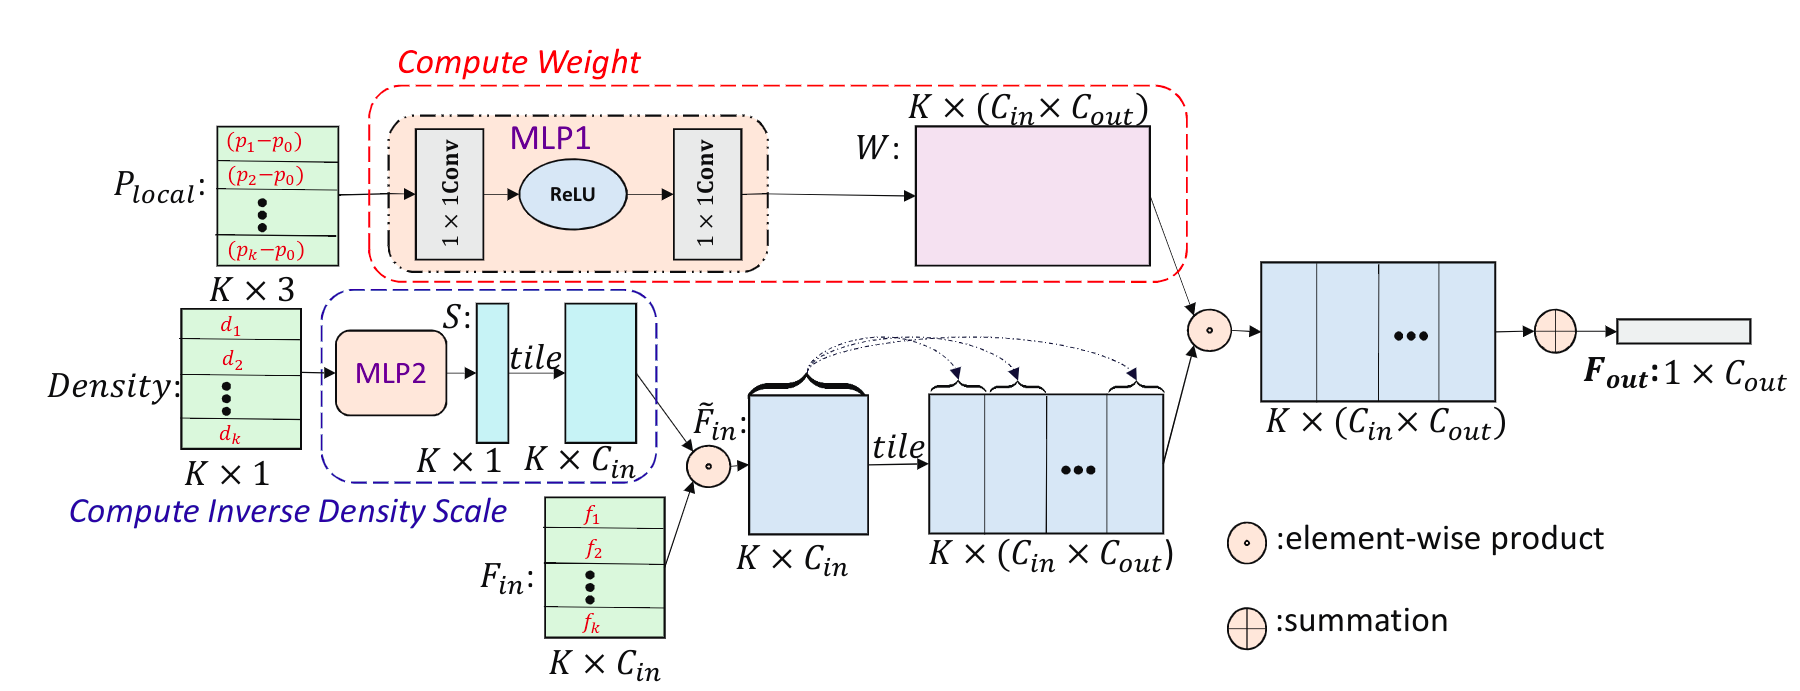
\includegraphics[width=\textwidth]{pointconv.png}
    \caption{PointConv operator~\cite{PointConv}}
    \label{fig:pointconvOperator}
\end{figure}

The weight function $W$ can be approximated by MLPs, while the density function, which outputs a value indicating how much points are concentrated around the centroid region, is calculated using kernel density estimation (KDE), described in~\cite{Turlach_bandwidthselection}, and then by appling a non-linear transform using an MLP.

The inputs of the PointConv operator are:

\begin{itemize}
    \item The subset of points $P_{local} \in \mathbb{R}^{K \times 3}$ : given a point $p_0$ in the point cloud, the $K$ closest points are taken and then the $p_0$ coordinates are subtracted to each point, obtaining the local coordinates of each point.
    \item The $ Density \in \mathbb{R} ^{K}$ estimated at each local point using KDE.
    \item The features $F_{in} \in \mathbb{R}^{K \times C_{in}}$, where $C_{in}$ is the number of channels, and for each channel there are the features associated with each local point. These features can be the point coordinates $(x, y, z)$, but also other features associated with the point such as the RGB color.
\end{itemize}

The \textit{Compute Weight} module is made by an MLP implemented as a $1 \times 1$ convolution, followed by a non-linear ReLU activation function, followed by another $1 \times 1$. The output of this module is $W \in \mathbb{R}^{K \times (C_{in} \times C_{out}})$.

The \textit{Compute Inverse Density Scale} module is used to calculate $S$: this is done by feeding the $Density$ into an MLP for a one dimensional linear transform. In this way the network can "decide" to use the density estimates.

Finally, the $F_{out} \in \mathbb{R}^{C_{out}}$ feature(s) associated with the feature(s) $F_{in}$ is:

\begin{equation}\label{eq:pointconv_orig}
\mathbf{F}_{\text {out }}=\sum_{k=1}^{K} \sum_{c_{i n}=1}^{C_{i n}} S(k) \mathbf{W}\left(k, c_{i n}\right) F_{i n}\left(k, c_{i n}\right)
\end{equation}

\paragraph{Architecture of a NN using PointConv} The architecture proposed in combination with PointConv is a hierarchical structure, composed by \textit{feature encoding blocks}. In each feature encoding block there is a sampling layer, a grouping layer and a PointConv. This feature encoding blocks (apart from the PointConv operator) are very similar to the ones already seen in PointNet++~\cite{qi2017pointnet++}, see also paragraph~\ref{par:pointnet++}. The only difference is that the neighbors of the centroid are calculated using the k-NN approach. In total the neural network is composed of 3 feature encoding blocks followed by 3 fully connected layers\footnote{See the code hosted on GitHub: \url{https://github.com/DylanWusee/pointconv_pytorch/blob/master/model/pointconv.py}}.

\paragraph{Efficient PointConv} A noticeable problem of the original PointConv operator is the memory needed for the $W$ function: given the batch size $B$, the number of points in the point cloud $N$, the number of local points $K$, the number of input channels $C_{in}$ and the number of output channels $C_{out}$ the size of the filter weight would be $B \times N \times K \times C_{in} \times C_{out}$.

It can be shown that PointConv equation~\ref{eq:pointconv_orig} can be reduced to a matrix multiplication and a 2D convolution. The new operator can be seen in figure~\ref{fig:efficientPointconv}. This can reduce the memory consumption by a factor of $1 / 64$.

\begin{figure}[ht]
    \centering
    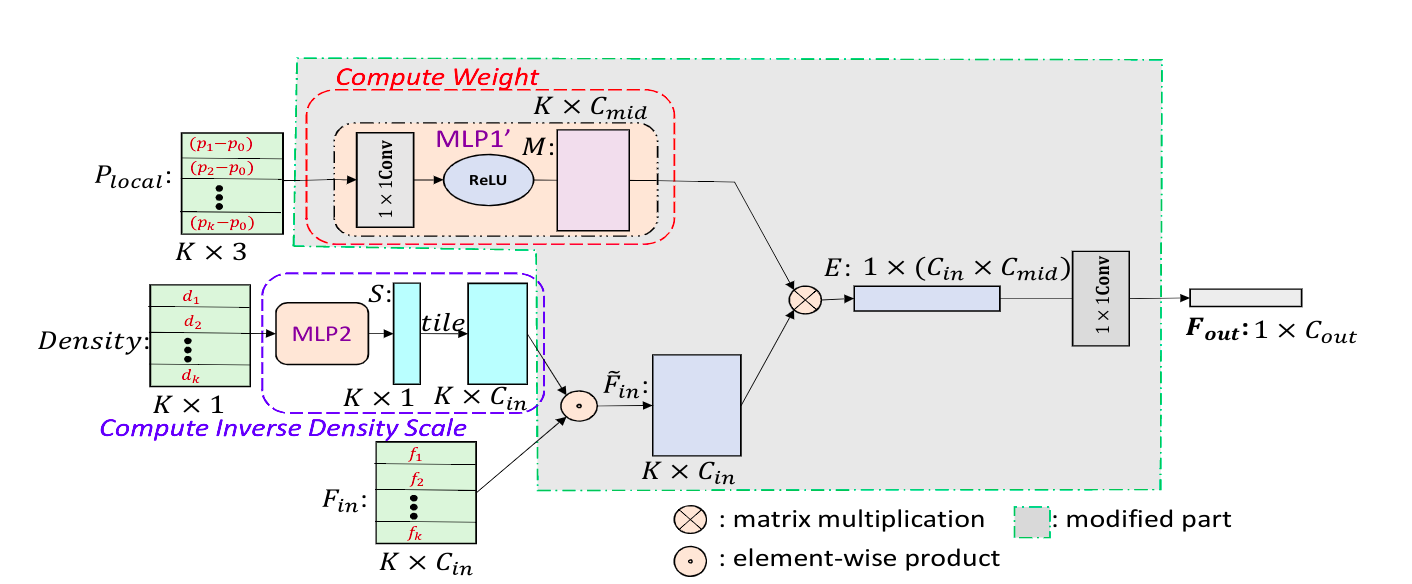
\includegraphics[width=\textwidth]{efficient_pointconv.png}
    \caption{Efficient PointConv~\cite{PointConv}}
    \label{fig:efficientPointconv}
\end{figure}

\paragraph{PointConv experiments}

The experiments have been performed on the ModelNet40 dataset, and have been conducted in the same way as PointNet authors did, which have become a standard to have a meaningful comparison between different networks. The overall accuracy obtained by PointConv on this dataset is $92.5$

An interesting experiment that has been carried out is the classification of CIFAR-10 dataset~\cite{Krizhevsky09learningmultiple}, which consists of 60000 32x32 colour images in 10 classes, with 6000 images per class. To demonstrate that PointConv is a good approximation of convolution the authors converted each point in an image into $(x,y)$ coordinates with the associated RGB color. Two CNNs have been trained, using PointConv as the convolution operator. The accuracy results in table~\ref{tab:pointconv_exp_cifar10} show that the networks using PointConv have roughly the same accuracy as normal CNNs, given that the overall architecture remains the same.

\begin{table}[ht]
    \centering
    \caption{CIFAR-10 experiments}
    \begin{tabular}{cc}
        \hline \text { Network } & \text { Accuracy (\%) } \\
        \hline AlexNet~\cite{AlexNet} & 89.00 \\
        VGG19~\cite{vgg19} & 93.60 \\
        \hline
        PointConv (5-layers) & 89.13 \\
        PointConv (VGG19) & 93.19 \\
        \hline
    \end{tabular}
    \label{tab:pointconv_exp_cifar10}
\end{table}